%------------------------------------------------------------------------
\begin{frame}
\frametitle{WebStorage}
\framesubtitle{Client Side Storage}
\begin{columns}[T] % align columns
\begin{column}{.48\textwidth}

\begin{center}
{\Huge WebStorage}
\end{center}

\end{column}%
\hfill%
\begin{column}{.48\textwidth}
\color{blue}\rule{\linewidth}{4pt}

	\setbeamertemplate{enumerate items}[default]
	\begin{enumerate}
		\item Same Origin Policy (SOP)
		\item Cookies
		\item \textbf{WebStorage}
		\item Application Cache
		\item IndexedDB
	\end{enumerate}
\end{column}%
\end{columns}
\end{frame}
%------------------------------------------------------------------------

\begin{frame}
\frametitle{WebStorage Fakten}
\framesubtitle{Client Side Storage}
	Webstorage (Supercookies)
	\begin{itemize}
		\item Key-Value Speicher
		\item W3C Proposed Recommendation
		\item Ursprünglich Teil des HTML5 Entwurfs
		\item Manche Browser bieten API um WebStorage als Objekt-, BLOB-Speicher an, jedoch internes mapping auf Strings!
		\item Speicherung erfolgt im DOM
	\end{itemize}
	\begin{textblock*}{3cm}(8cm,7cm) % {block width} (coords)
		
\includegraphics[height=3cm,width=3cm]{img/SuperCookie.png}
	\end{textblock*}
\end{frame}
%------------------------------------------------------------------------
\begin{frame}
\frametitle{WebStorage - Cookies}
\framesubtitle{Client Side Storage}
	Unterschied zu Cookies:
	\begin{itemize}
		\item $>$ 5 MB (1000 x)
		\item Rein clientseitig erzeugt und verwaltet
		\item Keine Versand in Requests/Responses
	\end{itemize}
\end{frame}
%------------------------------------------------------------------------
\begin{frame}
\frametitle{WebStorage}
\framesubtitle{Client Side Storage}
	WebStorage gliedert sich in:
	\begin{itemize}
		\item localStorage
		\begin{itemize}
			\item Erlaubt persistente Speicherung von Strings
			\item Speicherung ist zeitlich unbegrenzt
			\item SOP
		\end{itemize}
		\item sessionStorage
		\begin{itemize}
			\item Speicherung von Strings
			\item Lebenszeit auf das window Objekt begrenzt 
			\item Per-Origin-Per-Window
			\begin{itemize}
				\item Speicher auf window Objekt begrenzt
				\item Scripte in unterschiedlichen windows sind unabhängig \\
				$\rightarrow$ Trennung des Speichers trotz gleichem Origin	
			\end{itemize}
		\end{itemize}
	\end{itemize}
\end{frame}
%------------------------------------------------------------------------
\begin{frame}[fragile]
\frametitle{WebStorage}
\framesubtitle{Client Side Storage}
	WebStorage-API
	\begin{lstlisting}
	// Store value on browser for duration of the session
	sessionStorage.setItem('key', 'value');
		
	// Retrieve value 
	sessionStorage.getItem('key');
		
	// Store value on the browser beyond the duration of the session
	localStorage.setItem('key', 'value');
		
	// Retrieve value 
	localStorage.getItem('key');	
	\end{lstlisting}
\end{frame}
%------------------------------------------------------------------------
\begin{frame}[fragile]
\frametitle{WebStorage}
\framesubtitle{Client Side Storage}
	Speicherung von Objekten im localStorage:
	\begin{lstlisting}
	Storage.prototype.setObject = function(key, value) {
	    this.setItem(key, JSON.stringify(value));
	}
		
	Storage.prototype.getObject = function(key) {
	    var value = this.getItem(key);
		return value && JSON.parse(value);
	}
	\end{lstlisting}
\end{frame}
%------------------------------------------------------------------------
\begin{frame}[fragile]
\frametitle{WebStorage}
\framesubtitle{Client Side Storage}
	\begin{center}
		\large [Demo]
	\end{center}
\end{frame}
%------------------------------------------------------------------------
\begin{frame}[fragile]
\frametitle{WebStorage}
\framesubtitle{Client Side Storage}
	Browser Support
	\begin{center}
		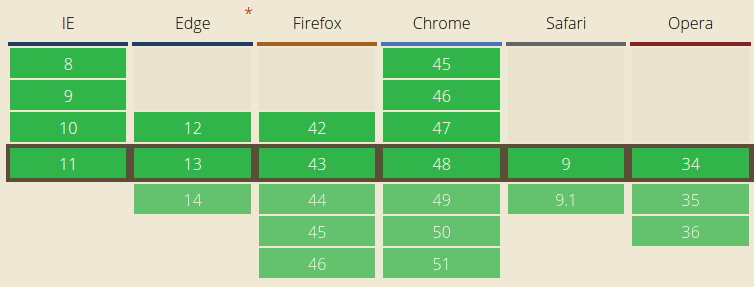
\includegraphics[height=5cm,width=11cm]{img/webStorage-support.png}
		\\
		
\includegraphics[height=0.5cm,width=5cm]{img/legende.png}
	\end{center}
\end{frame}